\hypertarget{IndependenceTest_8h}{
\section{IndependenceTest.h File Reference}
\label{IndependenceTest_8h}\index{IndependenceTest.h@{IndependenceTest.h}}
}


This graph shows which files directly or indirectly include this file:\nopagebreak
\begin{figure}[H]
\begin{center}
\leavevmode
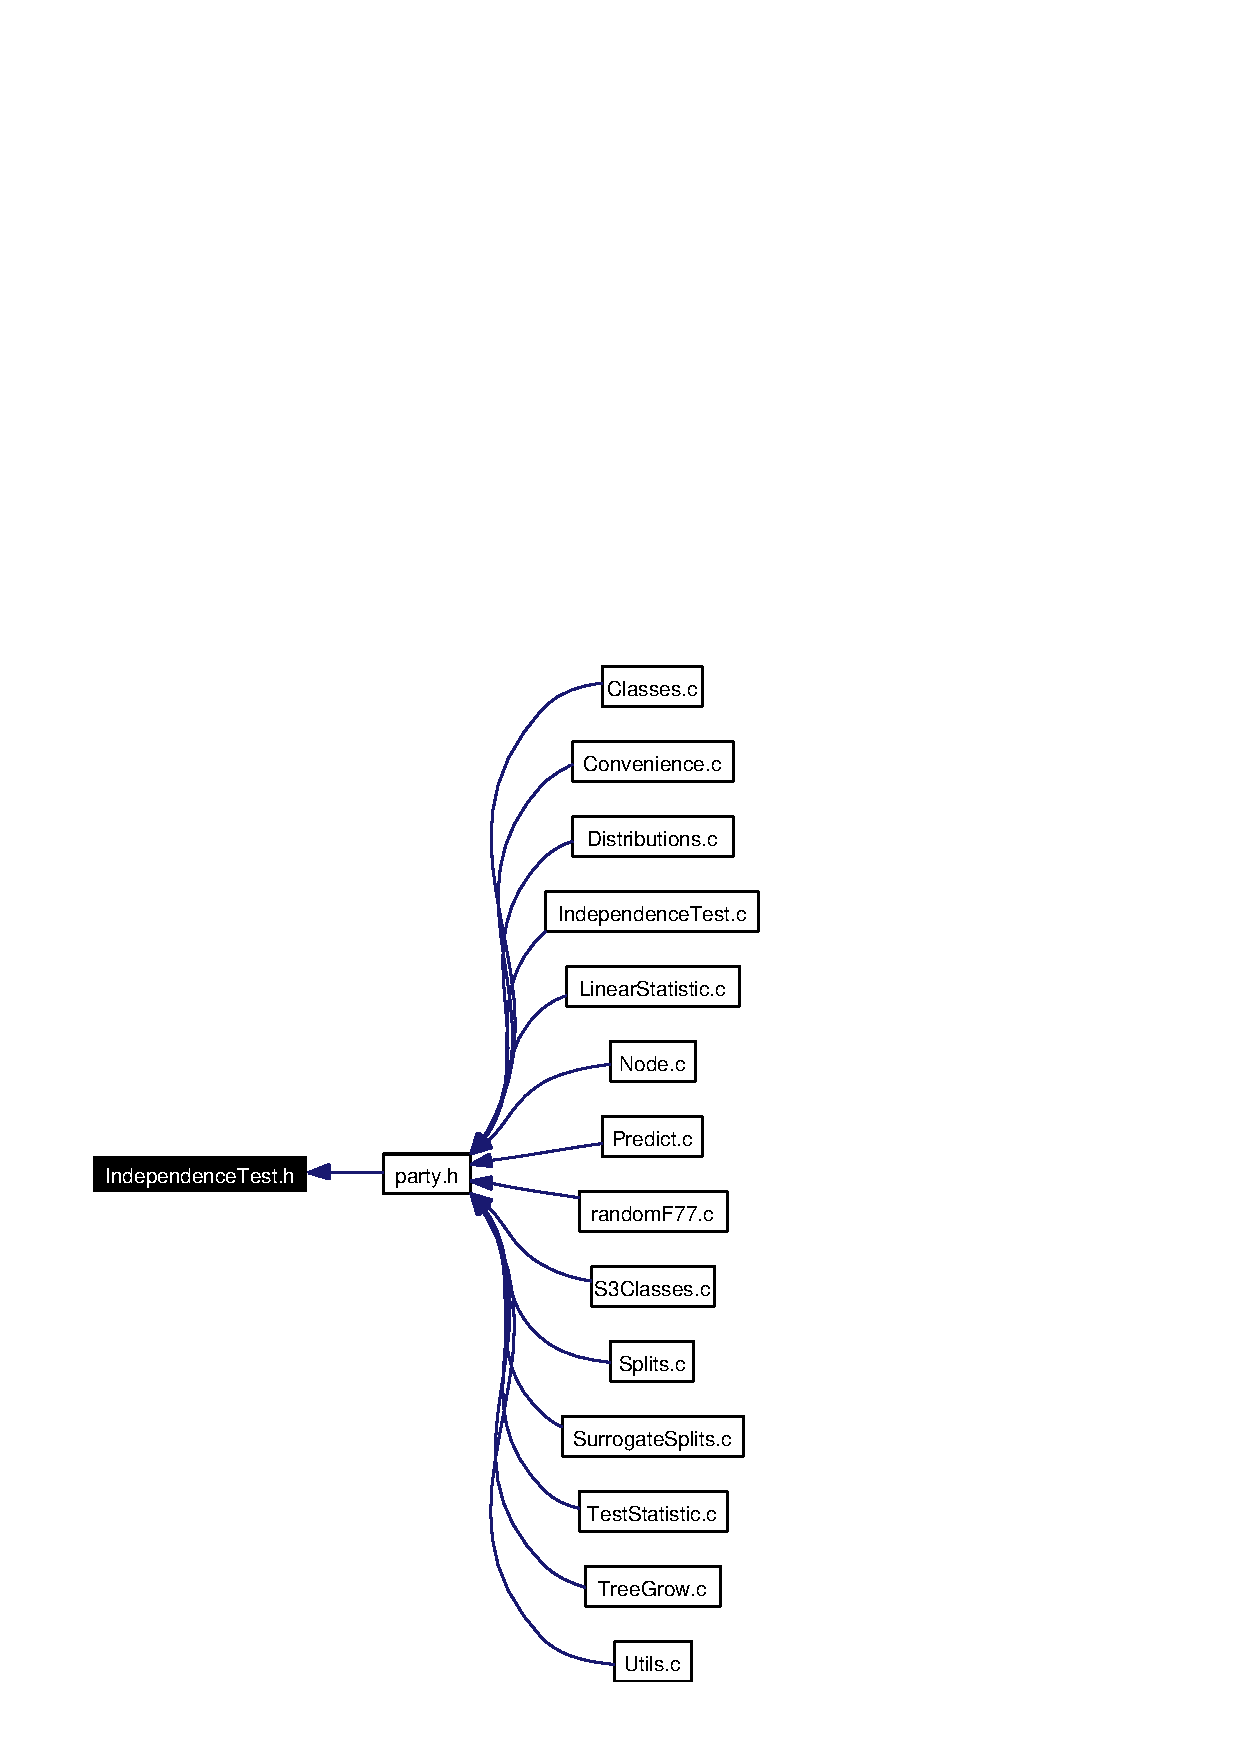
\includegraphics[width=420pt]{IndependenceTest_8h__dep__incl}
\end{center}
\end{figure}
\subsection*{Functions}
\begin{CompactItemize}
\item 
void \hyperlink{IndependenceTest_8h_cef73c662621fad56562bfc743025cc5}{C\_\-GlobalTest} (SEXP learnsample, SEXP weights, SEXP fitmem, SEXP varctrl, SEXP gtestctrl, double minsplit, double $\ast$teststat, double $\ast$criterion)
\item 
void \hyperlink{IndependenceTest_8h_b02275a67ad210d96fed9864590ee3ef}{C\_\-TeststatPvalue} (const SEXP linexpcov, const SEXP varctrl, double $\ast$ans\_\-teststat, double $\ast$ans\_\-pvalue)
\item 
void \hyperlink{IndependenceTest_8h_d33688ffc38df769a95d6964e5bb193a}{C\_\-TeststatCriterion} (const SEXP linexpcov, const SEXP varctrl, double $\ast$ans\_\-teststat, double $\ast$ans\_\-criterion)
\end{CompactItemize}


\subsection{Function Documentation}
\hypertarget{IndependenceTest_8h_cef73c662621fad56562bfc743025cc5}{
\index{IndependenceTest.h@{IndependenceTest.h}!C_GlobalTest@{C\_\-GlobalTest}}
\index{C_GlobalTest@{C\_\-GlobalTest}!IndependenceTest.h@{IndependenceTest.h}}
\subsubsection{\setlength{\rightskip}{0pt plus 5cm}void C\_\-GlobalTest (const SEXP {\em learnsample}, const SEXP {\em weights}, SEXP {\em fitmem}, const SEXP {\em varctrl}, const SEXP {\em gtctrl}, const double {\em minsplit}, double $\ast$ {\em ans\_\-teststat}, double $\ast$ {\em ans\_\-criterion})}}
\label{IndependenceTest_8h_cef73c662621fad56562bfc743025cc5}


Perform a global test on independence of a response and multiple inputs \par
 \begin{Desc}
\item[Parameters:]
\begin{description}
\item[{\em learnsample}]an object of class `LearningSample' \item[{\em weights}]case weights \item[{\em fitmem}]an object of class `TreeFitMemory' \item[{\em varctrl}]an object of class `VariableControl' \item[{\em gtctrl}]an object of class `GlobalTestControl' \item[{\em minsplit}]minimum sum of weights to proceed \item[{\em ans\_\-teststat}]return value; vector of test statistics \item[{\em ans\_\-criterion}]return value; vector of node criteria (adjusted) pvalues or raw test statistics \end{description}
\end{Desc}


Definition at line 129 of file IndependenceTest.c.

References AGGREGATED, BONFERRONI, C\_\-ExpectCovarInfluence(), C\_\-LinStatExpCov(), C\_\-LinStatExpCovMPinv(), C\_\-MonteCarlo(), C\_\-SampleNoReplace(), C\_\-tempweights(), C\_\-TeststatCriterion(), get\_\-dontuse(), get\_\-dontusetmp(), get\_\-mtry(), get\_\-ninputs(), get\_\-nobs(), get\_\-randomsplits(), get\_\-test\_\-trafo(), get\_\-teststat(), get\_\-testtype(), get\_\-tol(), get\_\-transformation(), get\_\-varmemory(), has\_\-missings(), MONTECARLO, ncol(), nrow(), PL2\_\-expcovinfSym, PL2\_\-inputsSym, PL2\_\-responsesSym, PL2\_\-sumweightsSym, TESTSTATISTIC, and UNIVARIATE.

Here is the call graph for this function:\nopagebreak
\begin{figure}[H]
\begin{center}
\leavevmode
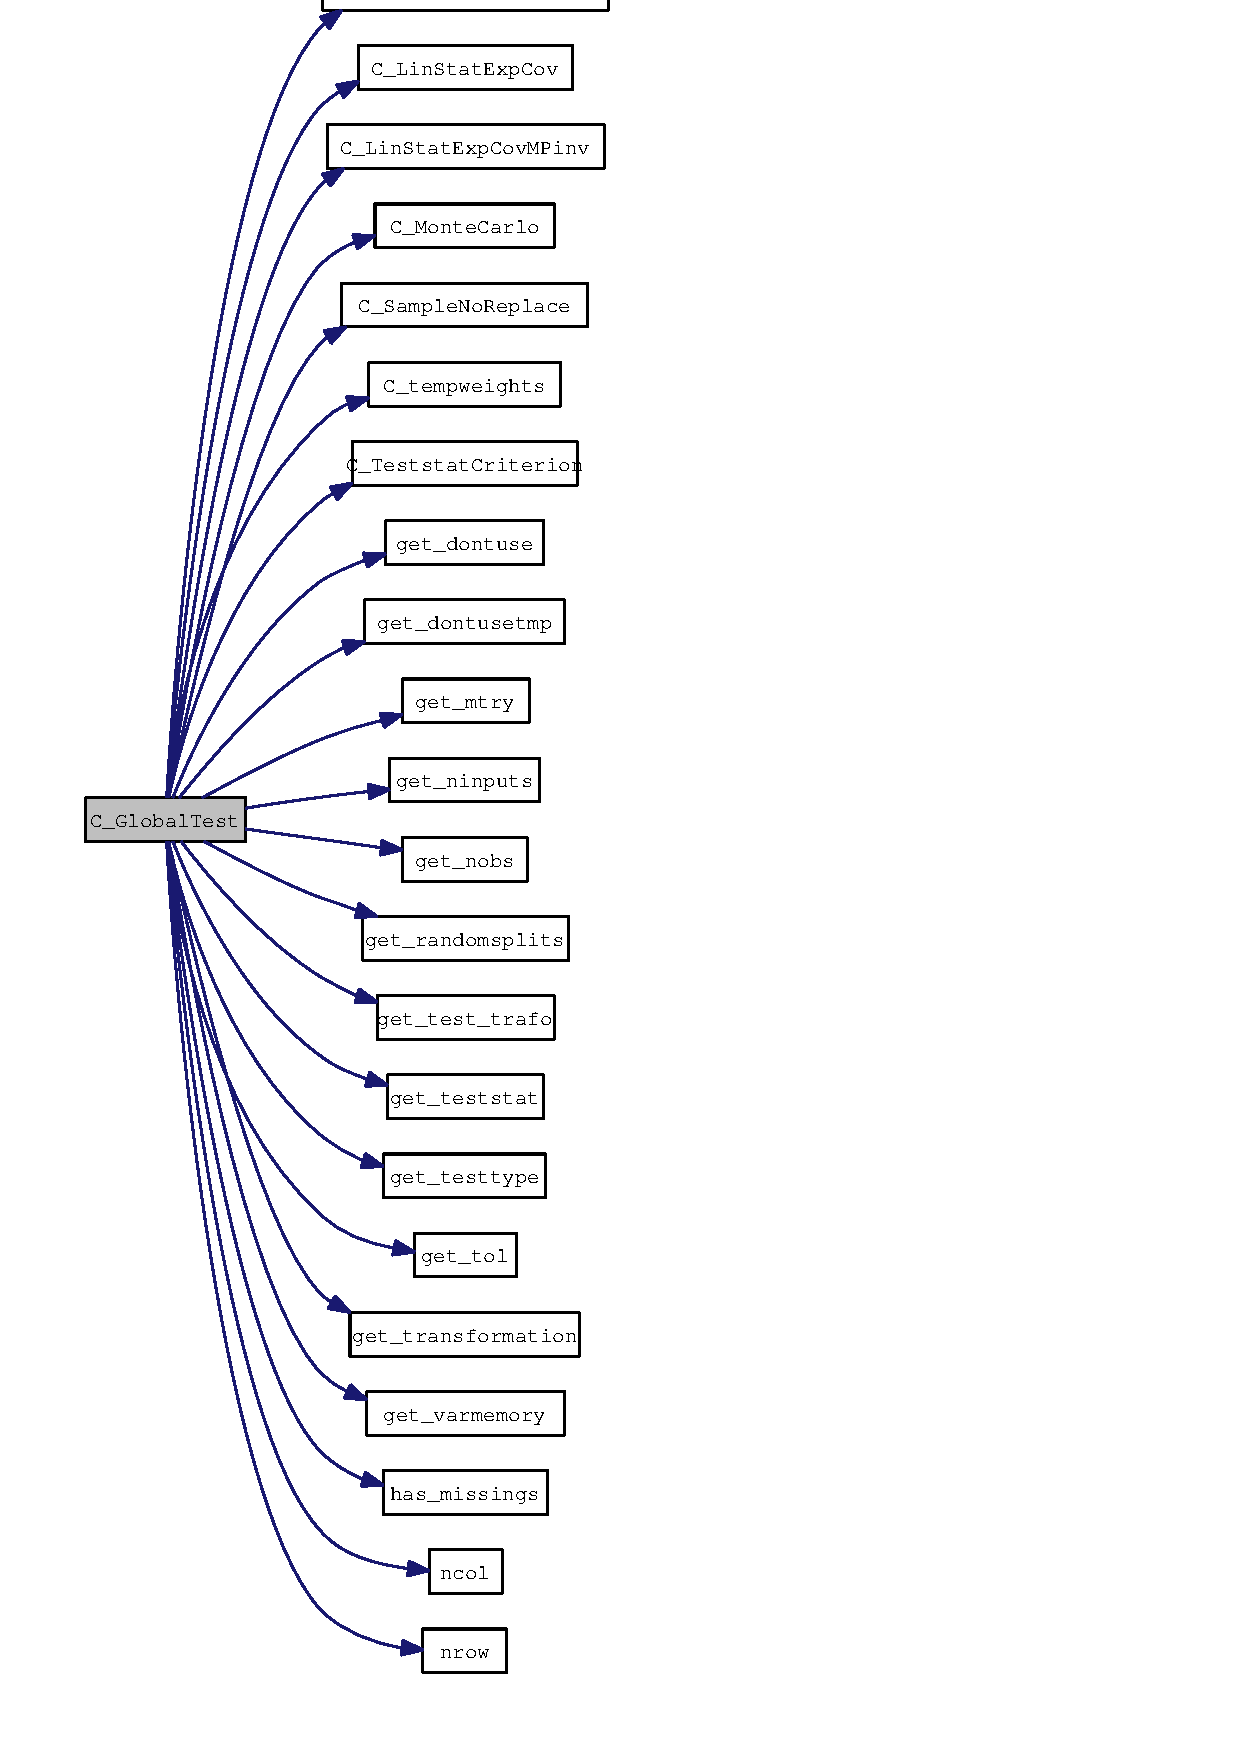
\includegraphics[width=148pt]{IndependenceTest_8h_cef73c662621fad56562bfc743025cc5_cgraph}
\end{center}
\end{figure}
\hypertarget{IndependenceTest_8h_d33688ffc38df769a95d6964e5bb193a}{
\index{IndependenceTest.h@{IndependenceTest.h}!C_TeststatCriterion@{C\_\-TeststatCriterion}}
\index{C_TeststatCriterion@{C\_\-TeststatCriterion}!IndependenceTest.h@{IndependenceTest.h}}
\subsubsection{\setlength{\rightskip}{0pt plus 5cm}void C\_\-TeststatCriterion (const SEXP {\em linexpcov}, const SEXP {\em varctrl}, double $\ast$ {\em ans\_\-teststat}, double $\ast$ {\em ans\_\-criterion})}}
\label{IndependenceTest_8h_d33688ffc38df769a95d6964e5bb193a}


Computes the test statistic and the node criterion \par
 \begin{Desc}
\item[Parameters:]
\begin{description}
\item[{\em linexpcov}]an object of class `LinStatExpectCovar' \item[{\em varctrl}]an object of class `VariableControl' \item[{\em ans\_\-teststat;}]return value, the test statistic \item[{\em ans\_\-criterion;}]return value, thep-value \end{description}
\end{Desc}


Definition at line 53 of file IndependenceTest.c.

References C\_\-TeststatPvalue(), and get\_\-pvalue().

Here is the call graph for this function:\nopagebreak
\begin{figure}[H]
\begin{center}
\leavevmode
\includegraphics[width=144pt]{IndependenceTest_8h_d33688ffc38df769a95d6964e5bb193a_cgraph}
\end{center}
\end{figure}
\hypertarget{IndependenceTest_8h_b02275a67ad210d96fed9864590ee3ef}{
\index{IndependenceTest.h@{IndependenceTest.h}!C_TeststatPvalue@{C\_\-TeststatPvalue}}
\index{C_TeststatPvalue@{C\_\-TeststatPvalue}!IndependenceTest.h@{IndependenceTest.h}}
\subsubsection{\setlength{\rightskip}{0pt plus 5cm}void C\_\-TeststatPvalue (const SEXP {\em linexpcov}, const SEXP {\em varctrl}, double $\ast$ {\em ans\_\-teststat}, double $\ast$ {\em ans\_\-pvalue})}}
\label{IndependenceTest_8h_b02275a67ad210d96fed9864590ee3ef}


Computes the test statistic and, if requested, the corresponding P-value for a linear statistic \par
 \begin{Desc}
\item[Parameters:]
\begin{description}
\item[{\em linexpcov}]an object of class `LinStatExpectCovar' \item[{\em varctrl}]an object of class `VariableControl' \item[{\em ans\_\-teststat;}]return value, the test statistic \item[{\em ans\_\-pvalue;}]return value, the p-value \end{description}
\end{Desc}


Definition at line 21 of file IndependenceTest.c.

References C\_\-ConditionalPvalue(), C\_\-TestStatistic(), get\_\-abseps(), get\_\-maxpts(), get\_\-pvalue(), get\_\-releps(), get\_\-teststat(), and get\_\-tol().

Here is the call graph for this function:\nopagebreak
\begin{figure}[H]
\begin{center}
\leavevmode
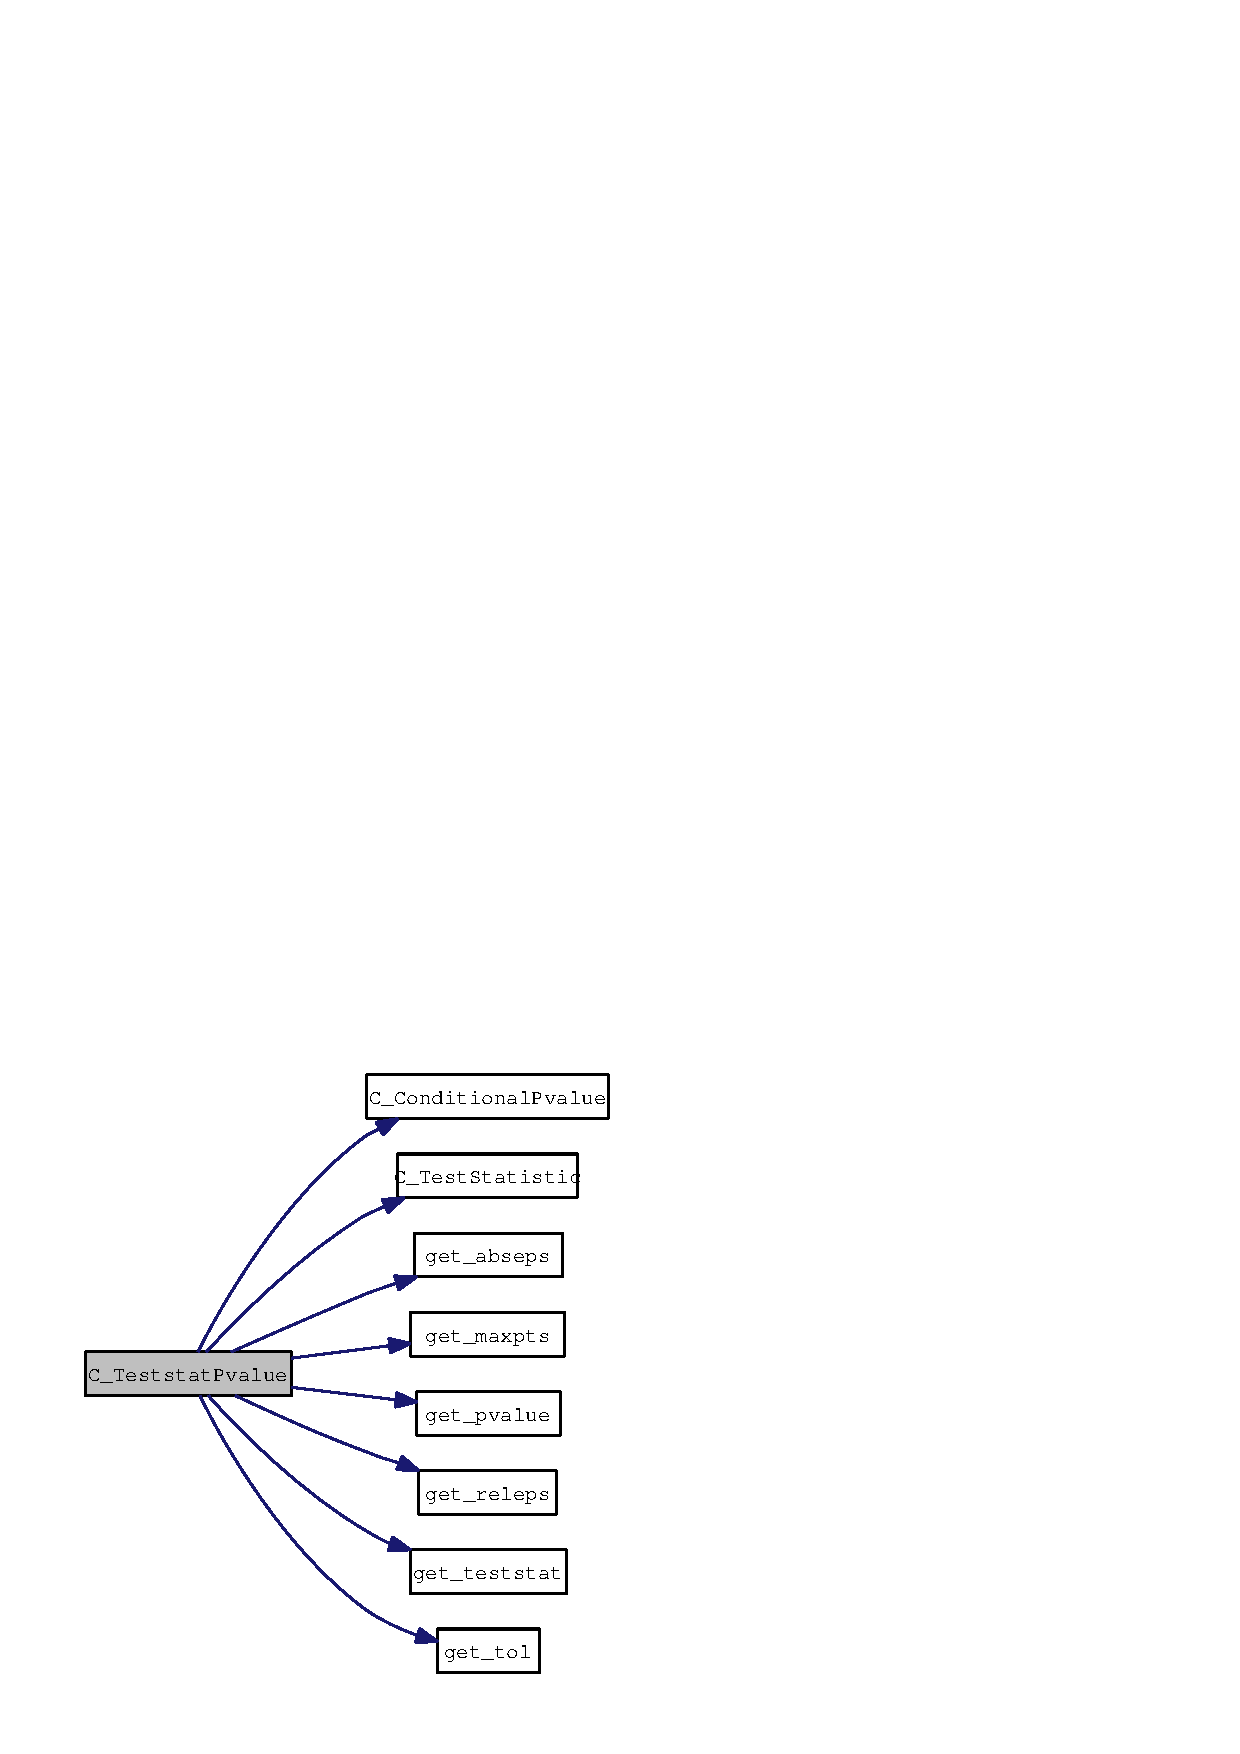
\includegraphics[width=148pt]{IndependenceTest_8h_b02275a67ad210d96fed9864590ee3ef_cgraph}
\end{center}
\end{figure}
